\chapter{Common Design and Implementation Strategy}\label{ch:design-implementation}


\section{Mechanism Model}\label{sec:mechanism-model}

After a thorough research and analysis of the available mechanisms implementations, it was identified the common design aspects that are shared among them.
These aspects, turned components, form the foundation of the future mechanisms implementations and are represented in the Mechanism Model, as shown in Figure~\ref{fig:mechanism-model}.

The Mechanism Model is composed of the following components:
\begin{itemize}
    \item \textbf{Configuration}: Represents a set of policies that, in conjuction, define the mechanism's behavior (e.g., maximum number of retries, maximum wait duration, etc.);
    \item \textbf{Asynchronous Context}: Represents the mechanism's execution context, responsible for state management and event emission;
    \item \textbf{State}: Represents the internal state of the mechanism;
    \item \textbf{Implementation}: Applies the configuration to the mechanism's execution context.
    Represents the core component of the mechanism;
    \item \textbf{Registry}: Acts as a centralized container for storing and managing available mechanism implementations and their configurations.
    The registry allows access to mechanism implementations throughout the application and enables the reuse of configurations to create new mechanisms.
    \item \textbf{Events}: Both the Asynchronous Context and Registry components are responsible for emitting events.
    The Asynchronous Context component emits events related to the mechanism's execution, such as internal state transition changes.
    The Registry component emits events related to CRUD operations (Create, Read, Update, Delete) performed in the registry.
    These events can be used for various purposes, such as logging and monitoring.
    \item \textbf{Metrics}: The mechanism's implementation component is responsible for recording metrics related to the mechanism's execution (e.g., number of retries, number of recorded failures, etc.).
    These metrics can be used for monitoring and analysis purposes.
    \item \textbf{Decorator}: The decorator is an extension of the Implementation component.
    It is based on Resilience4J~\cite{resilience4j} decorators (i.e., high-order functions), and provide a convenient way to wrap code blocks with the mechanism's behavior.
    \item \textbf{Ktor Plugin}: Responsible for the integration of the mechanism implementation with the Ktor pipeline.
    The Configuration component is also used to create a specific plugin configuration,
    which can be used to extend the mechanism's behavior and provide additional features in an HTTP context.
\end{itemize}

\begin{figure}
    \centering
    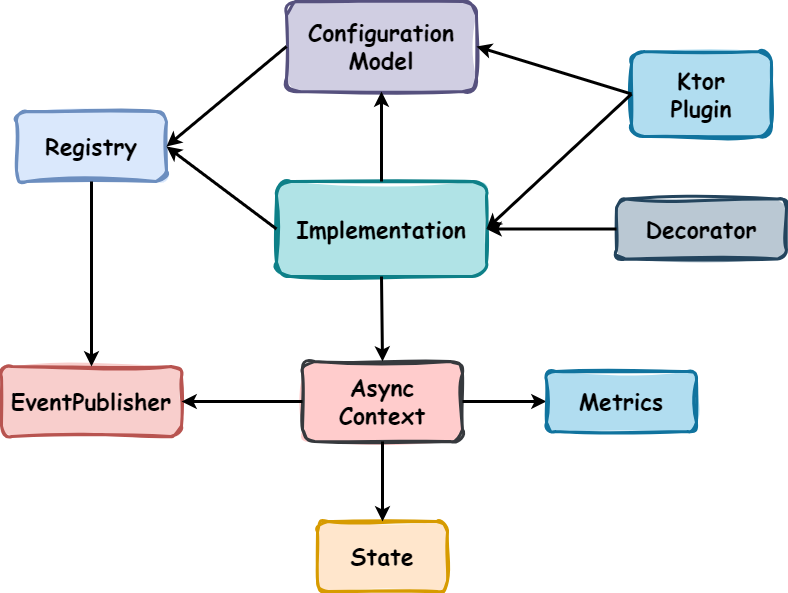
\includegraphics[width=0.8\textwidth]{../figures/03_mechanism-model}
    \caption{Mechanism Model}
    \label{fig:mechanism-model}
\end{figure}

\subsection{Configuration Design}\label{subsec:configuration-design}

Since the start of the project, the Configuration component was designed to use the builder pattern~\cite{wiki:builder-pattern}.
This way, separating the configuration definition (mutable) from the configuration usage (immutable).
However, the initial implementation had a limitation: it was not possible to override a configuration object (i.e., create a new configuration object based on an existing one and only change a few properties while keeping the rest).

In order to overcome this limitation, the Configuration component, and more specifically, its builder, was redesigned
to always receive a base configuration object in its creation.
This modification allows for incremental configuration, essentially following the pattern: \texttt{config(default/initial) -> configBuilder -> config -> configBuilder -> config -> (...)}~\ref{ch:appendix-config-builder}.

\subsection{Mechanism Execution Context}\label{subsec:mechanism-execution-context}

The mechanism's execution context is crucial for ensuring proper operation across synchronous and asynchronous environments.
Since the mechanisms are designed to be cross-platform, the execution context must be flexible and support asynchronous operations, particularly for JavaScript, one of the supported targets (see Section~\ref{sec:supported-targets}), which is single-threaded and requires asynchronous (non-blocking) operations.

Independent of the execution environment, the execution context is one of the following forms:

\begin{itemize}
    \item \textbf{Per Mechanism}: A new execution context is created when the mechanism itself is instantiated (e.g., the Circuit Breaker mechanism has a single execution context for managing the circuit state, as multiple callers can interact with the mechanism at the same time).
    \item \textbf{Per Decoration}: When a decorator is applied to an operation, it creates a new execution context specific to that decoration, before invoking the underlying operation.
    \item \textbf{Per Method Invocation}: A new execution context is created each time the decorated method is invoked.
    This is the most granular form of execution context, providing isolation for each method call.
    If the underlying operation is thread-safe, then this form of execution context is also thread-safe, as only the calling thread executes the context (e.g., the Retry mechanism creates a new execution context for each underlying operation invocation).
\end{itemize}


\section{Ktor Integration}\label{sec:ktor-integration}

talk about pipeline phase interception context


\section{Development Roadmap}\label{sec:development-roadmap}

Mechanism Model Implementation for a specific mechanism -> Tests -> All targets support -> Ktor plugin
and repeat for each mechanism in a vertical manner.
